

\chapter{Molecular Aggregates --- Coupled Two-Level Systems}



\section{Tasks}

\begin{itemize}
\item The data contains spectra and TCSPC traces of the molecule TDBC in solution at different concentrations. Determine the number of chromophores that contribute to the delocalized state,
\end{itemize}


%\section{Experiment}




\section{Coupled Pendulum}

A mathematical pendulum of point mass $m$ and rod length $L$ is governed by the differential equation of its angular displacement $\phi$
\[
 \ddot{\phi} + \frac{g}{L} \, \phi = 0 \quad \text{with} \quad \omega^2 = \frac{g}{l}
\]
where $g$ is the acceleration due to gravity and $\omega$ its angular eigen-frequency. When two of such pendula are coupled by a spring between the two masses, we get a coupled system of differential equations
\begin{eqnarray*}
 \ddot{\phi_1} + \frac{g}{L_1} \, \phi_1  + \frac{k}{m_1} \, \left( \phi_1  - \phi_2 \right)  & = &  0  \\
 \ddot{\phi_2} + \frac{g}{L_2} \, \phi_2  - \frac{k}{m_2} \, \left( \phi_1  - \phi_2 \right)  & = &  0  
\end{eqnarray*}
with the spring constant $k$.  For the moment, we assume that the pendula are identical, i.e., $L = L_1 = L_2$ and $m = m_1 =m_2$. The eigen-frequencies are then
\[
 \omega_{+}^2 = \frac{g}{L} \quad \text{and} \quad 
  \omega_{-}^2 = \frac{g}{L}  + 2 \frac{k}{m}
\]
where in the mode with frequency $\omega_{+}$ both masses move to the same direction, in the $\omega_{-}$ in opposite directions. Only in the latter case the coupling spring comes into play.

To investigate the general case, we assume harmonic oscillations, i.e. $\phi(t) = \phi_0 \, \exp (i \omega t)$ and write the differential equation as matrix
\[ \boldsymbol{M \, \phi}	 = 
\begin{pmatrix}
  \frac{g}{L_1} +  \frac{k}{m_1}&  - \frac{k}{m_1}\\
 - \frac{k}{m_2} &  \frac{g}{L_2} +  \frac{k}{m_2}
\end{pmatrix}  \boldsymbol{\phi}	= \omega^2   \, \boldsymbol{\phi}
\]
We thus search eigen-values and eigen-vectors of  $\boldsymbol{M}$. Assuming individual lengths, but identical masses, we get
\[
 \omega_{\pm}^2 = \left( \frac{\omega_1^2 + \omega_2^2}{2}  + \frac{k}{m} \right)
  \pm \sqrt{  \left( \frac{\omega_1^2 - \omega_2^2}{2}   \right)^2 + \left(  \frac{k}{m} \right)^2 }
\]
For identical lengths, i.e., identical eigen-frequencies $\omega_1 = \omega_2$, this recovers the results from above.


\section{Quantum Mechanics of Coupled States}

A quantum mechanical state is described by its eigen-function $\psi_a$ and the corresponding eigen-energy $E_a$ so that 
\[
\hat{H_a}  \, \psi_a = E_a  \,\psi_a  \quad .
\]
When we have two of such states, we can  write matrix equation
\[
\hat{H}_0 \, \psi_0 = \begin{pmatrix}  E_a & 0 \\ 0 & E_b \end{pmatrix} \,
	 \begin{pmatrix}  \psi_ a\\ \psi_b\end{pmatrix}  \quad .
\]
The Hamilton operator $\hat{H}_0$ is thus described by a $2 \times 2$ matrix. When the two states $a$ and $b$ are coupled, then the energy of one states depends somehow on the other. In the matrix we include a coupling energy $\beta$ in the off-diagonal elements
\[
\hat{H}_{coupled}  = \begin{pmatrix}  E_a & \beta \\ \beta & E_b \end{pmatrix} 
\]
As a consequence, the original eigen-functions $\psi_0$ are no longer eigen-functions of this coupled Hamilton operator. We find new eigen-functions and eigen-values by diagonalizing $\hat{H}_{coupled}$, so that the diagonal elements become
\[
 E_\pm = \frac{E_a + E_b}{2} \pm \sqrt{ \left( \frac{E_a - E_b}{2} \right)^2 + \beta^2 }
\]
and the new (not normalized) eigen-functions are\sidenote{A more symmetrical equation is given  in \cite{Parson}}
\[
 \psi_{\pm} = \psi_b + \psi_a \left[ \frac{E_a - E_b}{2 \beta} \pm \sqrt{ \left( \frac{E_a - E_b}{2 \beta} \right)^2 + 1  } \, \right]
\]
We can distinguish two limiting cases. The coupling energy $\beta$ can be larger than die energy difference between the two states, i.e. $\beta \gg |E_a - E_b| / 2$. Then then new eigen-energies are split up by $\pm \beta$ around the average of the old eigen-energies $(E_a + E_b) /2$. The eigen-functions in this situation are symmetric and anti-symmetric combinations of the old eigen-function, i.e. $\psi_\pm = \pm \psi_a + \psi_b$. When the coupling energy is small, i.e. $\beta \ll |E_a - E_b| / 2$, then the new eigen-energies and eigen-functions are close to the old.



\begin{figure}
   \includestandalone[width=10cm]{\currfiledir anticrossing}
\caption{Eigen-Energies and weights of the eigen-functions as function of the unperturbed energies ($E_b = 1$).}
\end{figure}

\textit{If coupling is EM wave, this is AC Stark effect}

\textit{time-dependence after preparation of a state}

\textit{include complex beta ?}


\section{Coupling of two transition dipole moments}


We consider two molecules, $a$ and $b$, each with a ground ($0$) and excited ($1$) state. We write the wave function on the form $\ket{ab}$, i.e. $\ket{01}$ is molecule $a$ in ground state, molecule $b$ in excited state. In each molecule, an optical transition diopole moment couples ground and excited state, i.e. $\braket{10| \hat{\mu}_a | 00}$ and $\braket{01| \hat{\mu}_b | 00}$ are different from zero and describe an excitation of the molecule  $a$ and $b$, respectively. Additionally, the two transition dipole moments interact and lead to a resonant coupling of the 
$\ket{01}$ and $\ket{10}$ state\footcite{knoester-book}
\[
\hat{H}_{coupling} = J \left(  \ket{10}\bra{01} + \ket{01}\bra{10}  \right)
\]
The coupling energy $J$ depends on distance $\boldsymbol{r}_{ab}$ and relative orientation of the transition dipoles $\boldsymbol{\mu}_{a,b}$. It can be seen as the energy of one dipole in the field of another\sidenote{does this need more details? See Parson}
\begin{eqnarray*}
 J & = & \frac{\boldsymbol{\mu}_a \cdot  \boldsymbol{\mu}_b }{|\boldsymbol{r}_{ab}|^3} 
  + 3 \frac{ (\boldsymbol{\mu}_a \cdot  \boldsymbol{r}_{ab})  (\boldsymbol{\mu}_b \cdot  \boldsymbol{r}_{ab})
  }{ |\boldsymbol{r}_{ab}|^5 } \\
   & = & \frac{\mu_a \mu_b }{r_{ab}^3} \left( \cos \theta - 3 \cos \alpha \, \cos \beta \right)  = \frac{\mu_a \mu_b }{r_{ab}^3} \, \kappa
\end{eqnarray*}
where the angles are defined in the sketch.\sidenote{NEEDS figure}


A similar coupling term also exist for the non-resonant coupling\footcite{knoester-book}
\[
\hat{H}_{non-res} = J \left(  \ket{11}\bra{00} + \ket{00}\bra{11}  \right)
\]
but this can be ignored, as it is non-resonant. All together, the Hamilton operator reads in matrix form
\[
\hat{H} = \begin{pmatrix}
0   					& \mu_a 						&	\mu_b						& 		J 		\\
\mu_a^\star	& \hbar \omega_a		&	J								& \mu_b	\\
\mu_b^\star  &  J^\star					& \hbar \omega_b		& \mu_a	\\
J^\star				& \mu_b^\star			& \mu_a^\star			& \hbar (\omega_a + \omega_b) \\
\end{pmatrix}
\]
When we ignore the double-excited state $\bra{11}$, the essence in contained in the center $2 \times 2$ matrix which we discussed already in the preceding section.

When $\ket{\psi}$ is a linear combination of $\ket{01}$ and $\ket{10}$, then also the transition dipole moment from $\ket{00}$ to $\ket{\psi}$ is a linear combination of $\mu_a$ and $\mu_b$ with the same weights. When $J \gg |E_a - E_b| / 2$ then we get
\[
 \boldsymbol{\mu}_{\pm} = \sqrt{1/2} \, \left( \boldsymbol{\mu}_a \pm  \boldsymbol{\mu}_b  \right) 
\]
The brightness of the absorption line is for identical molecules, i.e. $\mu = \mu_a = \mu_b$
\[
 I \propto |\boldsymbol{\mu}_{\pm}|^2 = (1/2) \, \left| \boldsymbol{\mu}_a \pm  \boldsymbol{\mu}_b  \right|^2 =  \left( 1 \pm \cos \theta \right) \, \left| \boldsymbol{\mu}   \right| ^2 
\]
where $\theta$ is as above the angle between the transition dipole moments. The same relation hold for the radiative rate.

The spectroscopic signature of coherent coupling between two molecules is thus a splitting of the absorption line into two lines, separated by twice the coupling energy $J$. The sum of the line amplitudes remains unchanged, but in some cases (J-aggregates, $\theta = 0$) one transition will take the whole amplitude and the other remains dark. In these cases, no splitting but a shift of the absorption line is observed. 

\begin{tabular}{llll}
$\theta$	&	$0^\circ$ & $90^\circ$ & $0^\circ$  \\
$\alpha$ & $0^\circ$ & $0^\circ$ & $90^\circ$  \\
$\beta$ & $0^\circ$ & $90^\circ$ & $90^\circ$  \\
$\kappa$  & $-2	$	& 	 $	0	$				& $1$   \\
\end{tabular}

needs vocabulary: Davydov splitting, cooperrative superradiance, H/J Aggregate

motional narrowing over inhom ensemble

ladder operator and more than 2 dipoles


%
%
%
%\section{Quantenmechanik gekoppelter Systeme\protect\footnote{Parson, Kap. 7.1 und 8.1, Stephan Wiesneth}} 
%
%
%
%Two molecules should be so close to each other that after excitation, it is no longer possible to determine which of the two molecules is excited. The excitation is thus delocalized via the system, which is also called \textit{exciton}. The exciton interaction does not physically differ from the interaction at resonance energy transfer.
%
%The state wave functions are again represented as a combination of the wave functions of the individual molecules:
%\[ \Psi_A = \phi_{1a}\chi_{1a}\phi_{2a}\chi_{2a} \]
%\[ \Psi_B = C_1\psi_1 + C_2\psi_2 = C_1\phi_{1b}\chi_{1b}\phi_{2a}\chi_{2a} + C_2\phi_{1a}\chi_{1a}\phi_{2b} \] 
%$\Psi_A$ corresponds to the basic state, $\Psi_B$ to the excited state of the dimmer. The $\psi_1$ and $\psi_2$ are not stationary states here, since the energy is quickly transferred back and forth between the molecules.
%
%The energy of the ground state is calculated as follows:
%\begin{equation}
%    E_A = \langle\phi_{1a}\phi_{2a}\lvert\tilde{H}_1+\tilde{H}_2+\tilde{H}'\rvert\phi_{1a}\phi_{2a}\rangle = E_{1a}+E_{2a}+\langle\phi_{1a}\phi_{2a}\lvert\tilde{H}'\rvert\phi_{1a}\phi_{2a}\rangle.
%\end{equation}
%The last term is very small compared to the first two if the molecules are uncharged and have a small transition dipole moment.
%
%For the energy of the excited state results
%\begin{equation}
%    E_B = \lvert C_1\rvert^2 E_1 + \lvert C_2\rvert^2 E_2 + \langle C_1\psi_1 + C_2\psi_2\lvert\tilde{H}'\rvert C_1\psi_1 + C_2\psi_2\rangle
%\end{equation}
%For a more precise calculation of the last term the stationary Schrödinger equation $\tilde{H}\Psi_B = E_B\Psi_B$ is used. This is multiplied once by $\psi_1*$ and once by $\psi_2*$. This gives the following system of equations:
%\[ C_1 \left [\langle\psi_1\lvert\tilde{H}_1\rvert\psi_1\rangle+\langle\psi_1\lvert\tilde{H}'\rvert\psi_1\rangle - E_B\right] + C_2\langle\psi_1\lvert\tilde{H}'\rvert\psi_2\rangle = 0 \]
%\[ C_1\langle\psi_2\lvert\tilde{H}'\rvert\psi_1\rangle + C_2 \left [\langle\psi_2\lvert\tilde{H}_2\rvert\psi_2\rangle+\langle\psi_2\lvert\tilde{H}'\rvert\psi_2\rangle - E_A\right] = 0 \]
%The non-trivial solution is obtained by equating the zero:
%\[ \begin{vmatrix}
%    H_{11} - E_A & H_{21} \\
%    H_{21} & H_{22} - E_B
%   \end{vmatrix} = 0 \] 
%Where $H_{11}=E_1+\langle\psi_1\lvert\tilde{H}'\rvert\psi_1\rangle$, corresponding for $H_{22}$ and $H_{21}=\langle\psi_2\lvert\tilde{H}'\rvert\psi_1\langle$. This gives you two possible values for $E_{B\pm}$, as well as two wave functions $\Psi_{B\pm}$:
%
%\begin{equation}
%    E_{B\pm} = E_0 \pm \frac{1}{2}\sqrt{\delta^2 + 4H_{12}^2}  
%\end{equation}
%\begin{equation}
%    \Psi_{B\pm} = \sqrt{\frac{1+s}{2}}\cdot\psi_1 \pm \sqrt{\frac{1-s}{2}}\cdot\psi_2
%\end{equation}
%The newly introduced variables are $\delta = H_{11}-H_{22}$, $E_0 = \frac{H_{11}+H_{22}}{2}$ and $s = \delta/\sqrt{\delta^2+4H_{21}^2}$. In a dimer the excited states of the individual molecules are thus split into two new energy levels.
%\begin{figure}
%    \centering
%    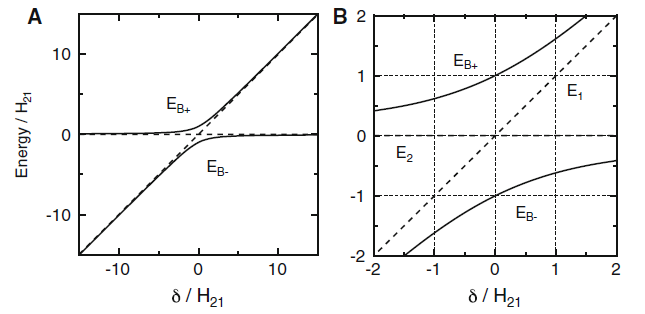
\includegraphics{\currfiledir/avoided_crossing.png}
%    \caption{Energies of the two new states depending on the energy difference of the single excited molecules}
%    \label{avoided_crossing}
%\end{figure}
%In figure \ref{avoided_crossing} it can be clearly seen that the energies of the states are never identical, which is also called \textit{avoided-crossing}.
%
%\section{Spectroscopy of dimers\protect\footnote{Parson, ch. 8.2}} 
%
%Which spectroscopic signature do coupled
%Fluorophores?
%
%\section{Antenna complexes\protect\footnote{Parson, section 8.5}} 
%
%In nature, coupled fluorophores are found in
%chlorophyll-antenna complexes. Why?




\printbibliography[segment=\therefsegment,heading=subbibliography]
